\documentclass[1p]{elsarticle_modified}
%\bibliographystyle{elsarticle-num}

%\usepackage[colorlinks]{hyperref}
%\usepackage{abbrmath_seonhwa} %\Abb, \Ascr, \Acal ,\Abf, \Afrak
\usepackage{amsfonts}
\usepackage{amssymb}
\usepackage{amsmath}
\usepackage{amsthm}
\usepackage{scalefnt}
\usepackage{amsbsy}
\usepackage{kotex}
\usepackage{caption}
\usepackage{subfig}
\usepackage{color}
\usepackage{graphicx}
\usepackage{xcolor} %% white, black, red, green, blue, cyan, magenta, yellow
\usepackage{float}
\usepackage{setspace}
\usepackage{hyperref}

\usepackage{tikz}
\usetikzlibrary{arrows}

\usepackage{multirow}
\usepackage{array} % fixed length table
\usepackage{hhline}

%%%%%%%%%%%%%%%%%%%%%
\makeatletter
\renewcommand*\env@matrix[1][\arraystretch]{%
	\edef\arraystretch{#1}%
	\hskip -\arraycolsep
	\let\@ifnextchar\new@ifnextchar
	\array{*\c@MaxMatrixCols c}}
\makeatother %https://tex.stackexchange.com/questions/14071/how-can-i-increase-the-line-spacing-in-a-matrix
%%%%%%%%%%%%%%%

\usepackage[normalem]{ulem}

\newcommand{\msout}[1]{\ifmmode\text{\sout{\ensuremath{#1}}}\else\sout{#1}\fi}
%SOURCE: \msout is \stkout macro in https://tex.stackexchange.com/questions/20609/strikeout-in-math-mode

\newcommand{\cancel}[1]{
	\ifmmode
	{\color{red}\msout{#1}}
	\else
	{\color{red}\sout{#1}}
	\fi
}

\newcommand{\add}[1]{
	{\color{blue}\uwave{#1}}
}

\newcommand{\replace}[2]{
	\ifmmode
	{\color{red}\msout{#1}}{\color{blue}\uwave{#2}}
	\else
	{\color{red}\sout{#1}}{\color{blue}\uwave{#2}}
	\fi
}

\newcommand{\Sol}{\mathcal{S}} %segment
\newcommand{\D}{D} %diagram
\newcommand{\A}{\mathcal{A}} %arc


%%%%%%%%%%%%%%%%%%%%%%%%%%%%%5 test

\def\sl{\operatorname{\textup{SL}}(2,\Cbb)}
\def\psl{\operatorname{\textup{PSL}}(2,\Cbb)}
\def\quan{\mkern 1mu \triangleright \mkern 1mu}

\theoremstyle{definition}
\newtheorem{thm}{Theorem}[section]
\newtheorem{prop}[thm]{Proposition}
\newtheorem{lem}[thm]{Lemma}
\newtheorem{ques}[thm]{Question}
\newtheorem{cor}[thm]{Corollary}
\newtheorem{defn}[thm]{Definition}
\newtheorem{exam}[thm]{Example}
\newtheorem{rmk}[thm]{Remark}
\newtheorem{alg}[thm]{Algorithm}

\newcommand{\I}{\sqrt{-1}}
\begin{document}

%\begin{frontmatter}
%
%\title{Boundary parabolic representations of knots up to 8 crossings}
%
%%% Group authors per affiliation:
%\author{Yunhi Cho} 
%\address{Department of Mathematics, University of Seoul, Seoul, Korea}
%\ead{yhcho@uos.ac.kr}
%
%
%\author{Seonhwa Kim} %\fnref{s_kim}}
%\address{Center for Geometry and Physics, Institute for Basic Science, Pohang, 37673, Korea}
%\ead{ryeona17@ibs.re.kr}
%
%\author{Hyuk Kim}
%\address{Department of Mathematical Sciences, Seoul National University, Seoul 08826, Korea}
%\ead{hyukkim@snu.ac.kr}
%
%\author{Seokbeom Yoon}
%\address{Department of Mathematical Sciences, Seoul National University, Seoul, 08826,  Korea}
%\ead{sbyoon15@snu.ac.kr}
%
%\begin{abstract}
%We find all boundary parabolic representation of knots up to 8 crossings.
%
%\end{abstract}
%\begin{keyword}
%    \MSC[2010] 57M25 
%\end{keyword}
%
%\end{frontmatter}

%\linenumbers
%\tableofcontents
%
\newcommand\colored[1]{\textcolor{white}{\rule[-0.35ex]{0.8em}{1.4ex}}\kern-0.8em\color{red} #1}%
%\newcommand\colored[1]{\textcolor{white}{ #1}\kern-2.17ex	\textcolor{white}{ #1}\kern-1.81ex	\textcolor{white}{ #1}\kern-2.15ex\color{red}#1	}

{\Large $\underline{12a_{1031}~(K12a_{1031})}$}

\setlength{\tabcolsep}{10pt}
\renewcommand{\arraystretch}{1.6}
\vspace{1cm}\begin{tabular}{m{100pt}>{\centering\arraybackslash}m{274pt}}
\multirow{5}{120pt}{
	\centering
	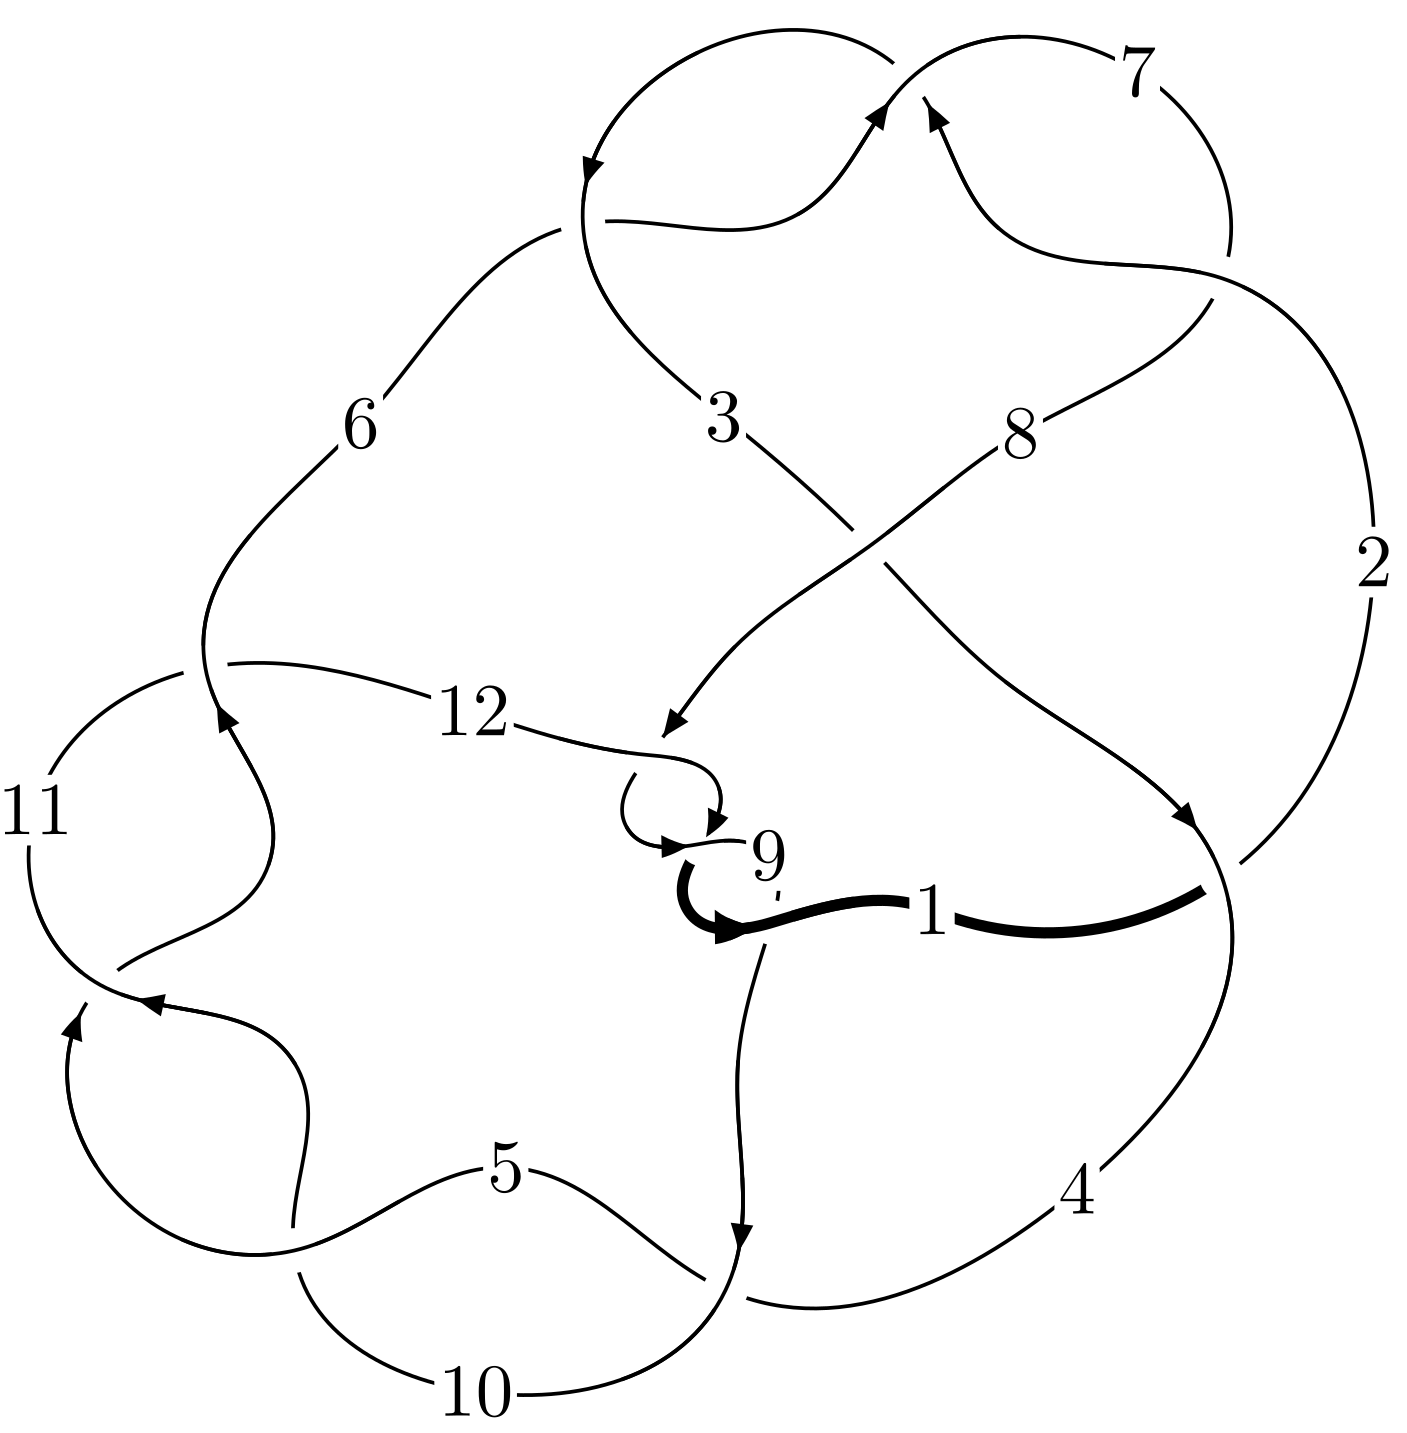
\includegraphics[width=112pt]{../../../GIT/diagram.site/Diagrams/png/1832_12a_1031.png}\\
\ \ \ A knot diagram\footnotemark}&
\allowdisplaybreaks
\textbf{Linearized knot diagam} \\
\cline{2-2}
 &
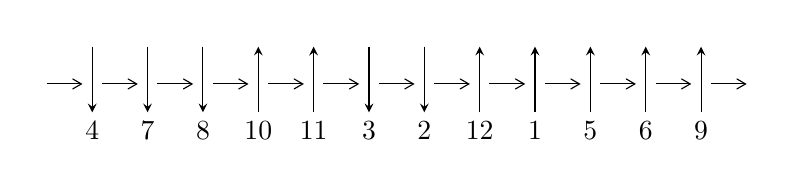
\begin{tikzpicture}[x=20pt, y=17pt]
	% nodes
	\node (C0) at (0, 0) {};
	\node (C1) at (1, 0) {};
	\node (C1U) at (1, +1) {};
	\node (C1D) at (1, -1) {4};

	\node (C2) at (2, 0) {};
	\node (C2U) at (2, +1) {};
	\node (C2D) at (2, -1) {7};

	\node (C3) at (3, 0) {};
	\node (C3U) at (3, +1) {};
	\node (C3D) at (3, -1) {8};

	\node (C4) at (4, 0) {};
	\node (C4U) at (4, +1) {};
	\node (C4D) at (4, -1) {10};

	\node (C5) at (5, 0) {};
	\node (C5U) at (5, +1) {};
	\node (C5D) at (5, -1) {11};

	\node (C6) at (6, 0) {};
	\node (C6U) at (6, +1) {};
	\node (C6D) at (6, -1) {3};

	\node (C7) at (7, 0) {};
	\node (C7U) at (7, +1) {};
	\node (C7D) at (7, -1) {2};

	\node (C8) at (8, 0) {};
	\node (C8U) at (8, +1) {};
	\node (C8D) at (8, -1) {12};

	\node (C9) at (9, 0) {};
	\node (C9U) at (9, +1) {};
	\node (C9D) at (9, -1) {1};

	\node (C10) at (10, 0) {};
	\node (C10U) at (10, +1) {};
	\node (C10D) at (10, -1) {5};

	\node (C11) at (11, 0) {};
	\node (C11U) at (11, +1) {};
	\node (C11D) at (11, -1) {6};

	\node (C12) at (12, 0) {};
	\node (C12U) at (12, +1) {};
	\node (C12D) at (12, -1) {9};
	\node (C13) at (13, 0) {};

	% arrows
	\draw[->,>={angle 60}]
	(C0) edge (C1) (C1) edge (C2) (C2) edge (C3) (C3) edge (C4) (C4) edge (C5) (C5) edge (C6) (C6) edge (C7) (C7) edge (C8) (C8) edge (C9) (C9) edge (C10) (C10) edge (C11) (C11) edge (C12) (C12) edge (C13) ;	\draw[->,>=stealth]
	(C1U) edge (C1D) (C2U) edge (C2D) (C3U) edge (C3D) (C4D) edge (C4U) (C5D) edge (C5U) (C6U) edge (C6D) (C7U) edge (C7D) (C8D) edge (C8U) (C9D) edge (C9U) (C10D) edge (C10U) (C11D) edge (C11U) (C12D) edge (C12U) ;
	\end{tikzpicture} \\
\hhline{~~} \\& 
\textbf{Solving Sequence} \\ \cline{2-2} 
 &
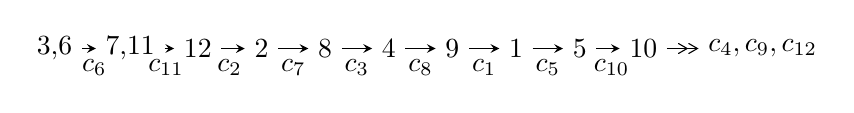
\begin{tikzpicture}[x=23pt, y=7pt]
	% node
	\node (A0) at (-1/8, 0) {3,6};
	\node (A1) at (17/16, 0) {7,11};
	\node (A2) at (17/8, 0) {12};
	\node (A3) at (25/8, 0) {2};
	\node (A4) at (33/8, 0) {8};
	\node (A5) at (41/8, 0) {4};
	\node (A6) at (49/8, 0) {9};
	\node (A7) at (57/8, 0) {1};
	\node (A8) at (65/8, 0) {5};
	\node (A9) at (73/8, 0) {10};
	\node (C1) at (1/2, -1) {$c_{6}$};
	\node (C2) at (13/8, -1) {$c_{11}$};
	\node (C3) at (21/8, -1) {$c_{2}$};
	\node (C4) at (29/8, -1) {$c_{7}$};
	\node (C5) at (37/8, -1) {$c_{3}$};
	\node (C6) at (45/8, -1) {$c_{8}$};
	\node (C7) at (53/8, -1) {$c_{1}$};
	\node (C8) at (61/8, -1) {$c_{5}$};
	\node (C9) at (69/8, -1) {$c_{10}$};
	\node (A10) at (11, 0) {$c_{4},c_{9},c_{12}$};

	% edge
	\draw[->,>=stealth]	
	(A0) edge (A1) (A1) edge (A2) (A2) edge (A3) (A3) edge (A4) (A4) edge (A5) (A5) edge (A6) (A6) edge (A7) (A7) edge (A8) (A8) edge (A9) ;
	\draw[->>,>={angle 60}]	
	(A9) edge (A10);
\end{tikzpicture} \\ 

\end{tabular} \\

\footnotetext{
The image of knot diagram is generated by the software ``\textbf{Draw programme}" developed by Andrew Bartholomew(\url{http://www.layer8.co.uk/maths/draw/index.htm\#Running-draw}), where we modified some parts for our purpose(\url{https://github.com/CATsTAILs/LinksPainter}).
}\phantom \\ \newline 
\centering \textbf{Ideals for irreducible components\footnotemark of $X_{\text{par}}$} 
 
\begin{align*}
I^u_{1}&=\langle 
-2.19647\times10^{18} u^{56}-5.09545\times10^{18} u^{55}+\cdots+7.20554\times10^{18} b+1.28415\times10^{19},\\
\phantom{I^u_{1}}&\phantom{= \langle  }-7.29984\times10^{18} u^{56}-1.44902\times10^{19} u^{55}+\cdots+7.20554\times10^{18} a+7.38518\times10^{19},\;u^{57}+2 u^{56}+\cdots-8 u+1\rangle \\
I^u_{2}&=\langle 
- u^2 a- u^2+b- a+u-2,\;2 u^2 a+a^2+u^2+2 a-3 u+2,\;u^3- u^2+2 u-1\rangle \\
I^u_{3}&=\langle 
b,\;- u^2+a-1,\;u^3+u^2+2 u+1\rangle \\
\\
\end{align*}
\raggedright * 3 irreducible components of $\dim_{\mathbb{C}}=0$, with total 66 representations.\\
\footnotetext{All coefficients of polynomials are rational numbers. But the coefficients are sometimes approximated in decimal forms when there is not enough margin.}
\newpage
\renewcommand{\arraystretch}{1}
\centering \section*{I. $I^u_{1}= \langle -2.20\times10^{18} u^{56}-5.10\times10^{18} u^{55}+\cdots+7.21\times10^{18} b+1.28\times10^{19},\;-7.30\times10^{18} u^{56}-1.45\times10^{19} u^{55}+\cdots+7.21\times10^{18} a+7.39\times10^{19},\;u^{57}+2 u^{56}+\cdots-8 u+1 \rangle$}
\flushleft \textbf{(i) Arc colorings}\\
\begin{tabular}{m{7pt} m{180pt} m{7pt} m{180pt} }
\flushright $a_{3}=$&$\begin{pmatrix}0\\u\end{pmatrix}$ \\
\flushright $a_{6}=$&$\begin{pmatrix}1\\0\end{pmatrix}$ \\
\flushright $a_{7}=$&$\begin{pmatrix}1\\u^2\end{pmatrix}$ \\
\flushright $a_{11}=$&$\begin{pmatrix}1.01309 u^{56}+2.01098 u^{55}+\cdots+4.60352 u-10.2493\\0.304830 u^{56}+0.707157 u^{55}+\cdots+1.30428 u-1.78217\end{pmatrix}$ \\
\flushright $a_{12}=$&$\begin{pmatrix}1.31792 u^{56}+2.71814 u^{55}+\cdots+5.90780 u-12.0315\\0.304830 u^{56}+0.707157 u^{55}+\cdots+1.30428 u-1.78217\end{pmatrix}$ \\
\flushright $a_{2}=$&$\begin{pmatrix}u\\u^3+u\end{pmatrix}$ \\
\flushright $a_{8}=$&$\begin{pmatrix}u^2+1\\u^4+2 u^2\end{pmatrix}$ \\
\flushright $a_{4}=$&$\begin{pmatrix}- u^5-2 u^3- u\\- u^7-3 u^5-2 u^3+u\end{pmatrix}$ \\
\flushright $a_{9}=$&$\begin{pmatrix}1.63554 u^{56}+3.51891 u^{55}+\cdots+6.76669 u-12.1033\\0.230341 u^{56}+0.550285 u^{55}+\cdots-0.632533 u-1.56754\end{pmatrix}$ \\
\flushright $a_{1}=$&$\begin{pmatrix}u^9+4 u^7+5 u^5+2 u^3+u\\u^{11}+5 u^9+8 u^7+3 u^5- u^3+u\end{pmatrix}$ \\
\flushright $a_{5}=$&$\begin{pmatrix}-2.34155 u^{56}-5.04434 u^{55}+\cdots-6.58540 u+15.6235\\-0.327980 u^{56}-0.616638 u^{55}+\cdots+0.0250809 u+2.21226\end{pmatrix}$ \\
\flushright $a_{10}=$&$\begin{pmatrix}-1.69640 u^{56}-3.90320 u^{55}+\cdots-8.13650 u+12.0154\\-0.122593 u^{56}-0.0875092 u^{55}+\cdots+1.34475 u+1.30123\end{pmatrix}$\\&\end{tabular}
\flushleft \textbf{(ii) Obstruction class $= -1$}\\~\\
\flushleft \textbf{(iii) Cusp Shapes $= -\frac{6051548760743078920}{3602767560289372397} u^{56}-\frac{8079139122240889311}{3602767560289372397} u^{55}+\cdots+\frac{59050771530991937522}{3602767560289372397} u+\frac{45876737479885210010}{3602767560289372397}$}\\~\\
\newpage\renewcommand{\arraystretch}{1}
\flushleft \textbf{(iv) u-Polynomials at the component}\newline \\
\begin{tabular}{m{50pt}|m{274pt}}
Crossings & \hspace{64pt}u-Polynomials at each crossing \\
\hline $$\begin{aligned}c_{1}\end{aligned}$$&$\begin{aligned}
&u^{57}-10 u^{56}+\cdots+1976 u+97
\end{aligned}$\\
\hline $$\begin{aligned}c_{2},c_{6},c_{7}\end{aligned}$$&$\begin{aligned}
&u^{57}+2 u^{56}+\cdots-8 u+1
\end{aligned}$\\
\hline $$\begin{aligned}c_{3}\end{aligned}$$&$\begin{aligned}
&u^{57}-2 u^{56}+\cdots-7940 u+797
\end{aligned}$\\
\hline $$\begin{aligned}c_{4},c_{5},c_{10}\\c_{11}\end{aligned}$$&$\begin{aligned}
&u^{57}- u^{56}+\cdots+8 u-8
\end{aligned}$\\
\hline $$\begin{aligned}c_{8},c_{9},c_{12}\end{aligned}$$&$\begin{aligned}
&u^{57}-4 u^{56}+\cdots+53 u+7
\end{aligned}$\\
\hline
\end{tabular}\\~\\
\newpage\renewcommand{\arraystretch}{1}
\flushleft \textbf{(v) Riley Polynomials at the component}\newline \\
\begin{tabular}{m{50pt}|m{274pt}}
Crossings & \hspace{64pt}Riley Polynomials at each crossing \\
\hline $$\begin{aligned}c_{1}\end{aligned}$$&$\begin{aligned}
&y^{57}+38 y^{56}+\cdots+7632286 y-9409
\end{aligned}$\\
\hline $$\begin{aligned}c_{2},c_{6},c_{7}\end{aligned}$$&$\begin{aligned}
&y^{57}+54 y^{56}+\cdots+70 y-1
\end{aligned}$\\
\hline $$\begin{aligned}c_{3}\end{aligned}$$&$\begin{aligned}
&y^{57}+14 y^{56}+\cdots+33141754 y-635209
\end{aligned}$\\
\hline $$\begin{aligned}c_{4},c_{5},c_{10}\\c_{11}\end{aligned}$$&$\begin{aligned}
&y^{57}-71 y^{56}+\cdots+960 y-64
\end{aligned}$\\
\hline $$\begin{aligned}c_{8},c_{9},c_{12}\end{aligned}$$&$\begin{aligned}
&y^{57}-60 y^{56}+\cdots+737 y-49
\end{aligned}$\\
\hline
\end{tabular}\\~\\
\newpage\flushleft \textbf{(vi) Complex Volumes and Cusp Shapes}
$$\begin{array}{c|c|c}  
\text{Solutions to }I^u_{1}& \I (\text{vol} + \sqrt{-1}CS) & \text{Cusp shape}\\
 \hline 
\begin{aligned}
u &= -0.587296 + 0.676990 I \\
a &= -0.992081 + 0.406961 I \\
b &= \phantom{-}1.68131 - 0.13190 I\end{aligned}
 & \phantom{-}16.3335 - 4.5705 I & \phantom{-}10.56013 + 0.39432 I \\ \hline\begin{aligned}
u &= -0.587296 - 0.676990 I \\
a &= -0.992081 - 0.406961 I \\
b &= \phantom{-}1.68131 + 0.13190 I\end{aligned}
 & \phantom{-}16.3335 + 4.5705 I & \phantom{-}10.56013 - 0.39432 I \\ \hline\begin{aligned}
u &= -0.774867 + 0.380193 I \\
a &= \phantom{-}0.56831 - 1.72511 I \\
b &= -1.67101 - 0.16539 I\end{aligned}
 & \phantom{-}15.3379 + 9.2274 I & \phantom{-}8.88615 - 5.62844 I \\ \hline\begin{aligned}
u &= -0.774867 - 0.380193 I \\
a &= \phantom{-}0.56831 + 1.72511 I \\
b &= -1.67101 + 0.16539 I\end{aligned}
 & \phantom{-}15.3379 - 9.2274 I & \phantom{-}8.88615 + 5.62844 I \\ \hline\begin{aligned}
u &= \phantom{-}0.831356\phantom{ +0.000000I} \\
a &= -0.649521\phantom{ +0.000000I} \\
b &= -1.63354\phantom{ +0.000000I}\end{aligned}
 & \phantom{-}9.95066\phantom{ +0.000000I} & \phantom{-}7.73730\phantom{ +0.000000I} \\ \hline\begin{aligned}
u &= \phantom{-}0.699421 + 0.384713 I \\
a &= -0.52691 - 1.35735 I \\
b &= \phantom{-}0.861493 - 0.565331 I\end{aligned}
 & \phantom{-}6.65268 - 6.38038 I & \phantom{-}7.53136 + 6.91744 I \\ \hline\begin{aligned}
u &= \phantom{-}0.699421 - 0.384713 I \\
a &= -0.52691 + 1.35735 I \\
b &= \phantom{-}0.861493 + 0.565331 I\end{aligned}
 & \phantom{-}6.65268 + 6.38038 I & \phantom{-}7.53136 - 6.91744 I \\ \hline\begin{aligned}
u &= -0.077518 + 1.200830 I \\
a &= -0.441853 + 0.527455 I \\
b &= \phantom{-}0.400809 + 0.440176 I\end{aligned}
 & \phantom{-}1.84442 + 1.53939 I & \phantom{-0.000000 } 0 \\ \hline\begin{aligned}
u &= -0.077518 - 1.200830 I \\
a &= -0.441853 - 0.527455 I \\
b &= \phantom{-}0.400809 - 0.440176 I\end{aligned}
 & \phantom{-}1.84442 - 1.53939 I & \phantom{-0.000000 } 0 \\ \hline\begin{aligned}
u &= -0.668942 + 0.396082 I \\
a &= -1.19802 + 1.74930 I \\
b &= \phantom{-}1.62450 + 0.07831 I\end{aligned}
 & \phantom{-}8.50640 + 4.83173 I & \phantom{-}6.80279 - 5.63364 I\\
 \hline 
 \end{array}$$\newpage$$\begin{array}{c|c|c}  
\text{Solutions to }I^u_{1}& \I (\text{vol} + \sqrt{-1}CS) & \text{Cusp shape}\\
 \hline 
\begin{aligned}
u &= -0.668942 - 0.396082 I \\
a &= -1.19802 - 1.74930 I \\
b &= \phantom{-}1.62450 - 0.07831 I\end{aligned}
 & \phantom{-}8.50640 - 4.83173 I & \phantom{-}6.80279 + 5.63364 I \\ \hline\begin{aligned}
u &= \phantom{-}0.540422 + 0.553317 I \\
a &= \phantom{-}0.0227086 + 0.0584366 I \\
b &= -0.926422 - 0.476199 I\end{aligned}
 & \phantom{-}7.32379 + 2.19374 I & \phantom{-}9.37328 - 0.81466 I \\ \hline\begin{aligned}
u &= \phantom{-}0.540422 - 0.553317 I \\
a &= \phantom{-}0.0227086 - 0.0584366 I \\
b &= -0.926422 + 0.476199 I\end{aligned}
 & \phantom{-}7.32379 - 2.19374 I & \phantom{-}9.37328 + 0.81466 I \\ \hline\begin{aligned}
u &= -0.558250 + 0.496865 I \\
a &= \phantom{-}1.63555 - 0.91390 I \\
b &= -1.61760 + 0.02546 I\end{aligned}
 & \phantom{-}8.95263 - 0.76794 I & \phantom{-}8.17007 - 0.54035 I \\ \hline\begin{aligned}
u &= -0.558250 - 0.496865 I \\
a &= \phantom{-}1.63555 + 0.91390 I \\
b &= -1.61760 - 0.02546 I\end{aligned}
 & \phantom{-}8.95263 + 0.76794 I & \phantom{-}8.17007 + 0.54035 I \\ \hline\begin{aligned}
u &= -0.271718 + 1.223630 I \\
a &= -0.099179 - 0.634045 I \\
b &= -0.666764 - 0.175562 I\end{aligned}
 & \phantom{-}5.53795 + 3.61211 I & \phantom{-0.000000 } 0 \\ \hline\begin{aligned}
u &= -0.271718 - 1.223630 I \\
a &= -0.099179 + 0.634045 I \\
b &= -0.666764 + 0.175562 I\end{aligned}
 & \phantom{-}5.53795 - 3.61211 I & \phantom{-0.000000 } 0 \\ \hline\begin{aligned}
u &= \phantom{-}0.206793 + 1.247570 I \\
a &= \phantom{-}1.18787 + 1.19469 I \\
b &= -1.46087 + 0.04757 I\end{aligned}
 & \phantom{-}7.77360 - 3.06996 I & \phantom{-0.000000 } 0 \\ \hline\begin{aligned}
u &= \phantom{-}0.206793 - 1.247570 I \\
a &= \phantom{-}1.18787 - 1.19469 I \\
b &= -1.46087 - 0.04757 I\end{aligned}
 & \phantom{-}7.77360 + 3.06996 I & \phantom{-0.000000 } 0 \\ \hline\begin{aligned}
u &= -0.601751 + 0.417912 I \\
a &= \phantom{-}0.568911 - 0.774796 I \\
b &= \phantom{-}0.064485 - 0.762242 I\end{aligned}
 & \phantom{-}4.25189 + 1.93714 I & \phantom{-}5.45403 - 3.24449 I\\
 \hline 
 \end{array}$$\newpage$$\begin{array}{c|c|c}  
\text{Solutions to }I^u_{1}& \I (\text{vol} + \sqrt{-1}CS) & \text{Cusp shape}\\
 \hline 
\begin{aligned}
u &= -0.601751 - 0.417912 I \\
a &= \phantom{-}0.568911 + 0.774796 I \\
b &= \phantom{-}0.064485 + 0.762242 I\end{aligned}
 & \phantom{-}4.25189 - 1.93714 I & \phantom{-}5.45403 + 3.24449 I \\ \hline\begin{aligned}
u &= \phantom{-}0.382994 + 1.209880 I \\
a &= -0.90161 - 1.11860 I \\
b &= \phantom{-}1.63564 - 0.03917 I\end{aligned}
 & \phantom{-}13.6861 - 4.3558 I & \phantom{-0.000000 } 0 \\ \hline\begin{aligned}
u &= \phantom{-}0.382994 - 1.209880 I \\
a &= -0.90161 + 1.11860 I \\
b &= \phantom{-}1.63564 + 0.03917 I\end{aligned}
 & \phantom{-}13.6861 + 4.3558 I & \phantom{-0.000000 } 0 \\ \hline\begin{aligned}
u &= -0.719732\phantom{ +0.000000I} \\
a &= \phantom{-}1.06954\phantom{ +0.000000I} \\
b &= \phantom{-}0.676169\phantom{ +0.000000I}\end{aligned}
 & \phantom{-}1.78784\phantom{ +0.000000I} & \phantom{-}6.76490\phantom{ +0.000000I} \\ \hline\begin{aligned}
u &= \phantom{-}0.089195 + 1.288090 I \\
a &= \phantom{-}1.043920 - 0.621762 I \\
b &= -0.408562 - 0.408532 I\end{aligned}
 & \phantom{-}4.90426 - 1.61227 I & \phantom{-0.000000 } 0 \\ \hline\begin{aligned}
u &= \phantom{-}0.089195 - 1.288090 I \\
a &= \phantom{-}1.043920 + 0.621762 I \\
b &= -0.408562 + 0.408532 I\end{aligned}
 & \phantom{-}4.90426 + 1.61227 I & \phantom{-0.000000 } 0 \\ \hline\begin{aligned}
u &= \phantom{-}0.597316 + 0.299927 I \\
a &= \phantom{-}0.75088 + 1.25022 I \\
b &= -0.698631 + 0.329985 I\end{aligned}
 & \phantom{-}0.45756 - 3.37876 I & \phantom{-}3.99050 + 8.66171 I \\ \hline\begin{aligned}
u &= \phantom{-}0.597316 - 0.299927 I \\
a &= \phantom{-}0.75088 - 1.25022 I \\
b &= -0.698631 - 0.329985 I\end{aligned}
 & \phantom{-}0.45756 + 3.37876 I & \phantom{-}3.99050 - 8.66171 I \\ \hline\begin{aligned}
u &= \phantom{-}0.027116 + 1.350160 I \\
a &= -2.00735 - 1.30623 I \\
b &= \phantom{-}1.43950 - 0.16113 I\end{aligned}
 & \phantom{-}10.95220 - 0.52770 I & \phantom{-0.000000 } 0 \\ \hline\begin{aligned}
u &= \phantom{-}0.027116 - 1.350160 I \\
a &= -2.00735 + 1.30623 I \\
b &= \phantom{-}1.43950 + 0.16113 I\end{aligned}
 & \phantom{-}10.95220 + 0.52770 I & \phantom{-0.000000 } 0\\
 \hline 
 \end{array}$$\newpage$$\begin{array}{c|c|c}  
\text{Solutions to }I^u_{1}& \I (\text{vol} + \sqrt{-1}CS) & \text{Cusp shape}\\
 \hline 
\begin{aligned}
u &= \phantom{-}0.636143\phantom{ +0.000000I} \\
a &= \phantom{-}0.899971\phantom{ +0.000000I} \\
b &= \phantom{-}1.45279\phantom{ +0.000000I}\end{aligned}
 & \phantom{-}3.96768\phantom{ +0.000000I} & -0.741900\phantom{ +0.000000I} \\ \hline\begin{aligned}
u &= -0.206696 + 1.359410 I \\
a &= \phantom{-}0.316733 + 0.033558 I \\
b &= \phantom{-}0.059845 - 0.466800 I\end{aligned}
 & \phantom{-}3.73122 + 3.46475 I & \phantom{-0.000000 } 0 \\ \hline\begin{aligned}
u &= -0.206696 - 1.359410 I \\
a &= \phantom{-}0.316733 - 0.033558 I \\
b &= \phantom{-}0.059845 + 0.466800 I\end{aligned}
 & \phantom{-}3.73122 - 3.46475 I & \phantom{-0.000000 } 0 \\ \hline\begin{aligned}
u &= \phantom{-}0.186663 + 1.395260 I \\
a &= \phantom{-}1.59178 + 0.51826 I \\
b &= -0.833776 - 0.025880 I\end{aligned}
 & \phantom{-}6.49247 - 1.98805 I & \phantom{-0.000000 } 0 \\ \hline\begin{aligned}
u &= \phantom{-}0.186663 - 1.395260 I \\
a &= \phantom{-}1.59178 - 0.51826 I \\
b &= -0.833776 + 0.025880 I\end{aligned}
 & \phantom{-}6.49247 + 1.98805 I & \phantom{-0.000000 } 0 \\ \hline\begin{aligned}
u &= \phantom{-}0.22801 + 1.41445 I \\
a &= -1.60611 - 0.79064 I \\
b &= \phantom{-}0.802162 - 0.369008 I\end{aligned}
 & \phantom{-}5.94609 - 6.40773 I & \phantom{-0.000000 } 0 \\ \hline\begin{aligned}
u &= \phantom{-}0.22801 - 1.41445 I \\
a &= -1.60611 + 0.79064 I \\
b &= \phantom{-}0.802162 + 0.369008 I\end{aligned}
 & \phantom{-}5.94609 + 6.40773 I & \phantom{-0.000000 } 0 \\ \hline\begin{aligned}
u &= -0.545024 + 0.153075 I \\
a &= -0.433814 + 0.605711 I \\
b &= -0.165016 + 0.402005 I\end{aligned}
 & -1.091470 + 0.719453 I & -4.41448 - 2.05784 I \\ \hline\begin{aligned}
u &= -0.545024 - 0.153075 I \\
a &= -0.433814 - 0.605711 I \\
b &= -0.165016 - 0.402005 I\end{aligned}
 & -1.091470 - 0.719453 I & -4.41448 + 2.05784 I \\ \hline\begin{aligned}
u &= -0.22391 + 1.45684 I \\
a &= -0.429922 - 0.136736 I \\
b &= -0.103875 + 0.846114 I\end{aligned}
 & \phantom{-}10.28030 + 4.97302 I & \phantom{-0.000000 } 0\\
 \hline 
 \end{array}$$\newpage$$\begin{array}{c|c|c}  
\text{Solutions to }I^u_{1}& \I (\text{vol} + \sqrt{-1}CS) & \text{Cusp shape}\\
 \hline 
\begin{aligned}
u &= -0.22391 - 1.45684 I \\
a &= -0.429922 + 0.136736 I \\
b &= -0.103875 - 0.846114 I\end{aligned}
 & \phantom{-}10.28030 - 4.97302 I & \phantom{-0.000000 } 0 \\ \hline\begin{aligned}
u &= -0.24951 + 1.45945 I \\
a &= \phantom{-}2.70655 - 1.58438 I \\
b &= -1.65433 - 0.10023 I\end{aligned}
 & \phantom{-}14.4830 + 8.1903 I & \phantom{-0.000000 } 0 \\ \hline\begin{aligned}
u &= -0.24951 - 1.45945 I \\
a &= \phantom{-}2.70655 + 1.58438 I \\
b &= -1.65433 + 0.10023 I\end{aligned}
 & \phantom{-}14.4830 - 8.1903 I & \phantom{-0.000000 } 0 \\ \hline\begin{aligned}
u &= \phantom{-}0.26230 + 1.45913 I \\
a &= \phantom{-}1.44999 + 0.74312 I \\
b &= -0.870143 + 0.634792 I\end{aligned}
 & \phantom{-}12.5896 - 9.8895 I & \phantom{-0.000000 } 0 \\ \hline\begin{aligned}
u &= \phantom{-}0.26230 - 1.45913 I \\
a &= \phantom{-}1.44999 - 0.74312 I \\
b &= -0.870143 - 0.634792 I\end{aligned}
 & \phantom{-}12.5896 + 9.8895 I & \phantom{-0.000000 } 0 \\ \hline\begin{aligned}
u &= -0.19701 + 1.46962 I \\
a &= -3.02622 + 0.91279 I \\
b &= \phantom{-}1.66182 + 0.00364 I\end{aligned}
 & \phantom{-}15.2659 + 1.9819 I & \phantom{-0.000000 } 0 \\ \hline\begin{aligned}
u &= -0.19701 - 1.46962 I \\
a &= -3.02622 - 0.91279 I \\
b &= \phantom{-}1.66182 - 0.00364 I\end{aligned}
 & \phantom{-}15.2659 - 1.9819 I & \phantom{-0.000000 } 0 \\ \hline\begin{aligned}
u &= \phantom{-}0.17782 + 1.47551 I \\
a &= -1.061720 - 0.450691 I \\
b &= \phantom{-}1.047880 + 0.514208 I\end{aligned}
 & \phantom{-}13.83430 - 0.35900 I & \phantom{-0.000000 } 0 \\ \hline\begin{aligned}
u &= \phantom{-}0.17782 - 1.47551 I \\
a &= -1.061720 + 0.450691 I \\
b &= \phantom{-}1.047880 - 0.514208 I\end{aligned}
 & \phantom{-}13.83430 + 0.35900 I & \phantom{-0.000000 } 0 \\ \hline\begin{aligned}
u &= \phantom{-}0.381646 + 0.332840 I \\
a &= -0.862209 - 0.317769 I \\
b &= \phantom{-}0.612157 + 0.106984 I\end{aligned}
 & \phantom{-}1.094310 + 0.315524 I & \phantom{-}8.13149 - 0.54452 I\\
 \hline 
 \end{array}$$\newpage$$\begin{array}{c|c|c}  
\text{Solutions to }I^u_{1}& \I (\text{vol} + \sqrt{-1}CS) & \text{Cusp shape}\\
 \hline 
\begin{aligned}
u &= \phantom{-}0.381646 - 0.332840 I \\
a &= -0.862209 + 0.317769 I \\
b &= \phantom{-}0.612157 - 0.106984 I\end{aligned}
 & \phantom{-}1.094310 - 0.315524 I & \phantom{-}8.13149 + 0.54452 I \\ \hline\begin{aligned}
u &= -0.29545 + 1.46817 I \\
a &= -2.14517 + 1.69345 I \\
b &= \phantom{-}1.67802 + 0.19089 I\end{aligned}
 & -18.1941 + 13.1223 I & \phantom{-0.000000 } 0 \\ \hline\begin{aligned}
u &= -0.29545 - 1.46817 I \\
a &= -2.14517 - 1.69345 I \\
b &= \phantom{-}1.67802 - 0.19089 I\end{aligned}
 & -18.1941 - 13.1223 I & \phantom{-0.000000 } 0 \\ \hline\begin{aligned}
u &= -0.14052 + 1.52399 I \\
a &= \phantom{-}2.53882 - 0.31091 I \\
b &= -1.72718 + 0.11615 I\end{aligned}
 & -15.8713 - 2.1155 I & \phantom{-0.000000 } 0 \\ \hline\begin{aligned}
u &= -0.14052 - 1.52399 I \\
a &= \phantom{-}2.53882 + 0.31091 I \\
b &= -1.72718 - 0.11615 I\end{aligned}
 & -15.8713 + 2.1155 I & \phantom{-0.000000 } 0 \\ \hline\begin{aligned}
u &= \phantom{-}0.357281\phantom{ +0.000000I} \\
a &= -1.94262\phantom{ +0.000000I} \\
b &= \phantom{-}0.364334\phantom{ +0.000000I}\end{aligned}
 & \phantom{-}1.04543\phantom{ +0.000000I} & \phantom{-}13.7800\phantom{ +0.000000I} \\ \hline\begin{aligned}
u &= \phantom{-}0.132476\phantom{ +0.000000I} \\
a &= -8.67705\phantom{ +0.000000I} \\
b &= -1.39067\phantom{ +0.000000I}\end{aligned}
 & \phantom{-}6.53451\phantom{ +0.000000I} & \phantom{-}14.2000\phantom{ +0.000000I}\\
 \hline 
 \end{array}$$\newpage\newpage\renewcommand{\arraystretch}{1}
\centering \section*{II. $I^u_{2}= \langle - u^2 a- u^2+b- a+u-2,\;2 u^2 a+a^2+u^2+2 a-3 u+2,\;u^3- u^2+2 u-1 \rangle$}
\flushleft \textbf{(i) Arc colorings}\\
\begin{tabular}{m{7pt} m{180pt} m{7pt} m{180pt} }
\flushright $a_{3}=$&$\begin{pmatrix}0\\u\end{pmatrix}$ \\
\flushright $a_{6}=$&$\begin{pmatrix}1\\0\end{pmatrix}$ \\
\flushright $a_{7}=$&$\begin{pmatrix}1\\u^2\end{pmatrix}$ \\
\flushright $a_{11}=$&$\begin{pmatrix}a\\u^2 a+u^2+a- u+2\end{pmatrix}$ \\
\flushright $a_{12}=$&$\begin{pmatrix}u^2 a+u^2+2 a- u+2\\u^2 a+u^2+a- u+2\end{pmatrix}$ \\
\flushright $a_{2}=$&$\begin{pmatrix}u\\u^2- u+1\end{pmatrix}$ \\
\flushright $a_{8}=$&$\begin{pmatrix}u^2+1\\u^2- u+1\end{pmatrix}$ \\
\flushright $a_{4}=$&$\begin{pmatrix}-1\\0\end{pmatrix}$ \\
\flushright $a_{9}=$&$\begin{pmatrix}- u^2 a-2 a+u-1\\- u^2 a- a-1\end{pmatrix}$ \\
\flushright $a_{1}=$&$\begin{pmatrix}u^2+1\\u^2- u+1\end{pmatrix}$ \\
\flushright $a_{5}=$&$\begin{pmatrix}- u^2 a+a u+u^2-2 a-2 u+1\\2\end{pmatrix}$ \\
\flushright $a_{10}=$&$\begin{pmatrix}- u^2 a- u^2-2 a+u-2\\- u^2 a- u^2- a+u-2\end{pmatrix}$\\&\end{tabular}
\flushleft \textbf{(ii) Obstruction class $= 1$}\\~\\
\flushleft \textbf{(iii) Cusp Shapes $= -4 u^2+4 u+4$}\\~\\
\newpage\renewcommand{\arraystretch}{1}
\flushleft \textbf{(iv) u-Polynomials at the component}\newline \\
\begin{tabular}{m{50pt}|m{274pt}}
Crossings & \hspace{64pt}u-Polynomials at each crossing \\
\hline $$\begin{aligned}c_{1}\end{aligned}$$&$\begin{aligned}
&(u^3+u^2-1)^2
\end{aligned}$\\
\hline $$\begin{aligned}c_{2}\end{aligned}$$&$\begin{aligned}
&(u^3+u^2+2 u+1)^2
\end{aligned}$\\
\hline $$\begin{aligned}c_{3}\end{aligned}$$&$\begin{aligned}
&(u^3- u^2+1)^2
\end{aligned}$\\
\hline $$\begin{aligned}c_{4},c_{5},c_{10}\\c_{11}\end{aligned}$$&$\begin{aligned}
&(u^2-2)^3
\end{aligned}$\\
\hline $$\begin{aligned}c_{6},c_{7}\end{aligned}$$&$\begin{aligned}
&(u^3- u^2+2 u-1)^2
\end{aligned}$\\
\hline $$\begin{aligned}c_{8},c_{9}\end{aligned}$$&$\begin{aligned}
&(u-1)^6
\end{aligned}$\\
\hline $$\begin{aligned}c_{12}\end{aligned}$$&$\begin{aligned}
&(u+1)^6
\end{aligned}$\\
\hline
\end{tabular}\\~\\
\newpage\renewcommand{\arraystretch}{1}
\flushleft \textbf{(v) Riley Polynomials at the component}\newline \\
\begin{tabular}{m{50pt}|m{274pt}}
Crossings & \hspace{64pt}Riley Polynomials at each crossing \\
\hline $$\begin{aligned}c_{1},c_{3}\end{aligned}$$&$\begin{aligned}
&(y^3- y^2+2 y-1)^2
\end{aligned}$\\
\hline $$\begin{aligned}c_{2},c_{6},c_{7}\end{aligned}$$&$\begin{aligned}
&(y^3+3 y^2+2 y-1)^2
\end{aligned}$\\
\hline $$\begin{aligned}c_{4},c_{5},c_{10}\\c_{11}\end{aligned}$$&$\begin{aligned}
&(y-2)^6
\end{aligned}$\\
\hline $$\begin{aligned}c_{8},c_{9},c_{12}\end{aligned}$$&$\begin{aligned}
&(y-1)^6
\end{aligned}$\\
\hline
\end{tabular}\\~\\
\newpage\flushleft \textbf{(vi) Complex Volumes and Cusp Shapes}
$$\begin{array}{c|c|c}  
\text{Solutions to }I^u_{2}& \I (\text{vol} + \sqrt{-1}CS) & \text{Cusp shape}\\
 \hline 
\begin{aligned}
u &= \phantom{-}0.215080 + 1.307140 I \\
a &= -0.57853 - 1.61567 I \\
b &= \phantom{-}1.41421\phantom{ +0.000000I}\end{aligned}
 & \phantom{-}9.60386 - 2.82812 I & \phantom{-}11.50976 + 2.97945 I \\ \hline\begin{aligned}
u &= \phantom{-}0.215080 + 1.307140 I \\
a &= \phantom{-}1.90324 + 0.49111 I \\
b &= -1.41421\phantom{ +0.000000I}\end{aligned}
 & \phantom{-}9.60386 - 2.82812 I & \phantom{-}11.50976 + 2.97945 I \\ \hline\begin{aligned}
u &= \phantom{-}0.215080 - 1.307140 I \\
a &= -0.57853 + 1.61567 I \\
b &= \phantom{-}1.41421\phantom{ +0.000000I}\end{aligned}
 & \phantom{-}9.60386 + 2.82812 I & \phantom{-}11.50976 - 2.97945 I \\ \hline\begin{aligned}
u &= \phantom{-}0.215080 - 1.307140 I \\
a &= \phantom{-}1.90324 - 0.49111 I \\
b &= -1.41421\phantom{ +0.000000I}\end{aligned}
 & \phantom{-}9.60386 + 2.82812 I & \phantom{-}11.50976 - 2.97945 I \\ \hline\begin{aligned}
u &= \phantom{-}0.569840\phantom{ +0.000000I} \\
a &= -0.257160\phantom{ +0.000000I} \\
b &= \phantom{-}1.41421\phantom{ +0.000000I}\end{aligned}
 & \phantom{-}5.46628\phantom{ +0.000000I} & \phantom{-}4.98050\phantom{ +0.000000I} \\ \hline\begin{aligned}
u &= \phantom{-}0.569840\phantom{ +0.000000I} \\
a &= -2.39228\phantom{ +0.000000I} \\
b &= -1.41421\phantom{ +0.000000I}\end{aligned}
 & \phantom{-}5.46628\phantom{ +0.000000I} & \phantom{-}4.98050\phantom{ +0.000000I}\\
 \hline 
 \end{array}$$\newpage\newpage\renewcommand{\arraystretch}{1}
\centering \section*{III. $I^u_{3}= \langle b,\;- u^2+a-1,\;u^3+u^2+2 u+1 \rangle$}
\flushleft \textbf{(i) Arc colorings}\\
\begin{tabular}{m{7pt} m{180pt} m{7pt} m{180pt} }
\flushright $a_{3}=$&$\begin{pmatrix}0\\u\end{pmatrix}$ \\
\flushright $a_{6}=$&$\begin{pmatrix}1\\0\end{pmatrix}$ \\
\flushright $a_{7}=$&$\begin{pmatrix}1\\u^2\end{pmatrix}$ \\
\flushright $a_{11}=$&$\begin{pmatrix}u^2+1\\0\end{pmatrix}$ \\
\flushright $a_{12}=$&$\begin{pmatrix}u^2+1\\0\end{pmatrix}$ \\
\flushright $a_{2}=$&$\begin{pmatrix}u\\- u^2- u-1\end{pmatrix}$ \\
\flushright $a_{8}=$&$\begin{pmatrix}u^2+1\\u^2+u+1\end{pmatrix}$ \\
\flushright $a_{4}=$&$\begin{pmatrix}1\\0\end{pmatrix}$ \\
\flushright $a_{9}=$&$\begin{pmatrix}2 u^2+2\\u^2+u+1\end{pmatrix}$ \\
\flushright $a_{1}=$&$\begin{pmatrix}- u^2-1\\- u^2- u-1\end{pmatrix}$ \\
\flushright $a_{5}=$&$\begin{pmatrix}1\\0\end{pmatrix}$ \\
\flushright $a_{10}=$&$\begin{pmatrix}u^2+1\\0\end{pmatrix}$\\&\end{tabular}
\flushleft \textbf{(ii) Obstruction class $= 1$}\\~\\
\flushleft \textbf{(iii) Cusp Shapes $= -6 u^2-4 u-4$}\\~\\
\newpage\renewcommand{\arraystretch}{1}
\flushleft \textbf{(iv) u-Polynomials at the component}\newline \\
\begin{tabular}{m{50pt}|m{274pt}}
Crossings & \hspace{64pt}u-Polynomials at each crossing \\
\hline $$\begin{aligned}c_{1},c_{3}\end{aligned}$$&$\begin{aligned}
&u^3+u^2-1
\end{aligned}$\\
\hline $$\begin{aligned}c_{2}\end{aligned}$$&$\begin{aligned}
&u^3- u^2+2 u-1
\end{aligned}$\\
\hline $$\begin{aligned}c_{4},c_{5},c_{10}\\c_{11}\end{aligned}$$&$\begin{aligned}
&u^3
\end{aligned}$\\
\hline $$\begin{aligned}c_{6},c_{7}\end{aligned}$$&$\begin{aligned}
&u^3+u^2+2 u+1
\end{aligned}$\\
\hline $$\begin{aligned}c_{8},c_{9}\end{aligned}$$&$\begin{aligned}
&(u+1)^3
\end{aligned}$\\
\hline $$\begin{aligned}c_{12}\end{aligned}$$&$\begin{aligned}
&(u-1)^3
\end{aligned}$\\
\hline
\end{tabular}\\~\\
\newpage\renewcommand{\arraystretch}{1}
\flushleft \textbf{(v) Riley Polynomials at the component}\newline \\
\begin{tabular}{m{50pt}|m{274pt}}
Crossings & \hspace{64pt}Riley Polynomials at each crossing \\
\hline $$\begin{aligned}c_{1},c_{3}\end{aligned}$$&$\begin{aligned}
&y^3- y^2+2 y-1
\end{aligned}$\\
\hline $$\begin{aligned}c_{2},c_{6},c_{7}\end{aligned}$$&$\begin{aligned}
&y^3+3 y^2+2 y-1
\end{aligned}$\\
\hline $$\begin{aligned}c_{4},c_{5},c_{10}\\c_{11}\end{aligned}$$&$\begin{aligned}
&y^3
\end{aligned}$\\
\hline $$\begin{aligned}c_{8},c_{9},c_{12}\end{aligned}$$&$\begin{aligned}
&(y-1)^3
\end{aligned}$\\
\hline
\end{tabular}\\~\\
\newpage\flushleft \textbf{(vi) Complex Volumes and Cusp Shapes}
$$\begin{array}{c|c|c}  
\text{Solutions to }I^u_{3}& \I (\text{vol} + \sqrt{-1}CS) & \text{Cusp shape}\\
 \hline 
\begin{aligned}
u &= -0.215080 + 1.307140 I \\
a &= -0.662359 - 0.562280 I \\
b &= \phantom{-0.000000 } 0\end{aligned}
 & \phantom{-}4.66906 + 2.82812 I & \phantom{-}6.83447 - 1.85489 I \\ \hline\begin{aligned}
u &= -0.215080 - 1.307140 I \\
a &= -0.662359 + 0.562280 I \\
b &= \phantom{-0.000000 } 0\end{aligned}
 & \phantom{-}4.66906 - 2.82812 I & \phantom{-}6.83447 + 1.85489 I \\ \hline\begin{aligned}
u &= -0.569840\phantom{ +0.000000I} \\
a &= \phantom{-}1.32472\phantom{ +0.000000I} \\
b &= \phantom{-0.000000 } 0\end{aligned}
 & \phantom{-}0.531480\phantom{ +0.000000I} & -3.66890\phantom{ +0.000000I}\\
 \hline 
 \end{array}$$\newpage
\newpage\renewcommand{\arraystretch}{1}
\centering \section*{ IV. u-Polynomials}
\begin{tabular}{m{50pt}|m{274pt}}
Crossings & \hspace{64pt}u-Polynomials at each crossing \\
\hline $$\begin{aligned}c_{1}\end{aligned}$$&$\begin{aligned}
&((u^3+u^2-1)^3)(u^{57}-10 u^{56}+\cdots+1976 u+97)
\end{aligned}$\\
\hline $$\begin{aligned}c_{2}\end{aligned}$$&$\begin{aligned}
&(u^3- u^2+2 u-1)(u^3+u^2+2 u+1)^2(u^{57}+2 u^{56}+\cdots-8 u+1)
\end{aligned}$\\
\hline $$\begin{aligned}c_{3}\end{aligned}$$&$\begin{aligned}
&((u^3- u^2+1)^2)(u^3+u^2-1)(u^{57}-2 u^{56}+\cdots-7940 u+797)
\end{aligned}$\\
\hline $$\begin{aligned}c_{4},c_{5},c_{10}\\c_{11}\end{aligned}$$&$\begin{aligned}
&u^3(u^2-2)^3(u^{57}- u^{56}+\cdots+8 u-8)
\end{aligned}$\\
\hline $$\begin{aligned}c_{6},c_{7}\end{aligned}$$&$\begin{aligned}
&((u^3- u^2+2 u-1)^2)(u^3+u^2+2 u+1)(u^{57}+2 u^{56}+\cdots-8 u+1)
\end{aligned}$\\
\hline $$\begin{aligned}c_{8},c_{9}\end{aligned}$$&$\begin{aligned}
&((u-1)^6)(u+1)^3(u^{57}-4 u^{56}+\cdots+53 u+7)
\end{aligned}$\\
\hline $$\begin{aligned}c_{12}\end{aligned}$$&$\begin{aligned}
&((u-1)^3)(u+1)^6(u^{57}-4 u^{56}+\cdots+53 u+7)
\end{aligned}$\\
\hline
\end{tabular}\newpage\renewcommand{\arraystretch}{1}
\centering \section*{ V. Riley Polynomials}
\begin{tabular}{m{50pt}|m{274pt}}
Crossings & \hspace{64pt}Riley Polynomials at each crossing \\
\hline $$\begin{aligned}c_{1}\end{aligned}$$&$\begin{aligned}
&((y^3- y^2+2 y-1)^3)(y^{57}+38 y^{56}+\cdots+7632286 y-9409)
\end{aligned}$\\
\hline $$\begin{aligned}c_{2},c_{6},c_{7}\end{aligned}$$&$\begin{aligned}
&((y^3+3 y^2+2 y-1)^3)(y^{57}+54 y^{56}+\cdots+70 y-1)
\end{aligned}$\\
\hline $$\begin{aligned}c_{3}\end{aligned}$$&$\begin{aligned}
&((y^3- y^2+2 y-1)^3)(y^{57}+14 y^{56}+\cdots+3.31418\times10^{7} y-635209)
\end{aligned}$\\
\hline $$\begin{aligned}c_{4},c_{5},c_{10}\\c_{11}\end{aligned}$$&$\begin{aligned}
&y^3(y-2)^6(y^{57}-71 y^{56}+\cdots+960 y-64)
\end{aligned}$\\
\hline $$\begin{aligned}c_{8},c_{9},c_{12}\end{aligned}$$&$\begin{aligned}
&((y-1)^9)(y^{57}-60 y^{56}+\cdots+737 y-49)
\end{aligned}$\\
\hline
\end{tabular}
\vskip 2pc
\end{document}